\begin{poster}{
    grid=false,
    headerborder=open,           % Adds a border around the header of content boxes
    colspacing=1em,              % Column spacing
    bgColorOne=white,            % Background color for the gradient on the left side of the poster
    bgColorTwo=white,            % Background color for the gradient on the right side of the poster
    borderColor=white,           % Border color
    headerColorOne=violet,       % Background color for the header in the content boxes (left side)
    headerColorTwo=white,        % Background color for the header in the content boxes (right side)
    headerFontColor=white,       % Text color for the header text in the content boxes
    boxColorOne=white,           % Background color of the content boxes
    textborder=rounded,          %rectangle, % Format of the border around content boxes, can be: none, bars, coils, triangles, rectangle, rounded, roundedsmall, roundedright or faded
    eyecatcher=false,            % Set to false for ignoring the left logo in the title and move the title left
    headerheight=0.1\textheight, % Height of the header
    headershape=rounded,         % Specify the rounded corner in the content box headers, can be: rectangle, small-rounded, roundedright, roundedleft or rounded
    headershade=plain,
    headerfont=\Large\textsf,    % Large, bold and sans serif font in the headers of content boxes
    %textfont={\setlength{\parindent}{1.5em}}, % Uncomment for paragraph indentation
    linewidth=2pt                % Width of the border lines around content boxes
}{
    
\includegraphics[scale=.3]{esiee}
}{
   \textsf{Smart Lora Transmission Parameters Selection}
}{
    \sf\vspace{0.2em}\\
    Aghiles DJOUDI\Mark{1}\Mark{2}, Rafik ZITOUNI\Mark{2}, Nawel ZANGAR\Mark{1} and Laurent GEORGE\Mark{1}
    \vspace{0.3em}\\
    \small{
        \Mark{1}LIGM/ESIEE Paris, 5 boulevard Descartes, Cité Descartes, Champs-sur-Marne, France\\
        \Mark{2}SIC/ECE Paris, 37 Quai de Grenelle, 75015 Paris, France
        \vspace{0.3em}\\
    }
    Email:   aghiles.djoudi@esiee.fr, rafik.zitouni@ece.fr, nawel.zangar@esiee.fr, laurent.george@esiee.fr

}{
    
\includegraphics[scale=.13]{esiee}
}


\headerbox{1. Introduction}{name=introduction,column=0,row=0, span=3}{
     The need of new kind of wireless communication that could send data far away with limited resource constraints emerged recently to support IoT application like smart building smart environment monitoring.
 \textbf{LoraWan} is one of this emerging wireless network \cite{ayoub_internet_22},
    it allows sensors to reach the gateway with start topology in a range up to 5Km.
Unlike other technologies LoraWan is the best versatile solution to deploy IoT application in both urban and rural area where there is no communication infrastructure.

}

\headerbox{2. Parameters selection problem}{name=mcs,column=0,below=introduction,span=1}{
    The physical layer of Lora technology (Semtech SX1276) has 4 parameters which make 6720 possible settings \cite{noura_interoperability_2018}:
    \begin{itemize}
        \item[\ding{224}] \textbf{SF:} Spreading factor [SF7 - SF12]
        \item[\ding{224}] \textbf{CR:} Coding rate [4/5 - 4/8]
        \item[\ding{224}] \textbf{BW:} Bandwidth [7.8Khz - 500Khz]
        \item[\ding{224}] \textbf{Tx:} Transmition power [-4dBm~+20dBm]
    \end{itemize}

    \begin{center}
        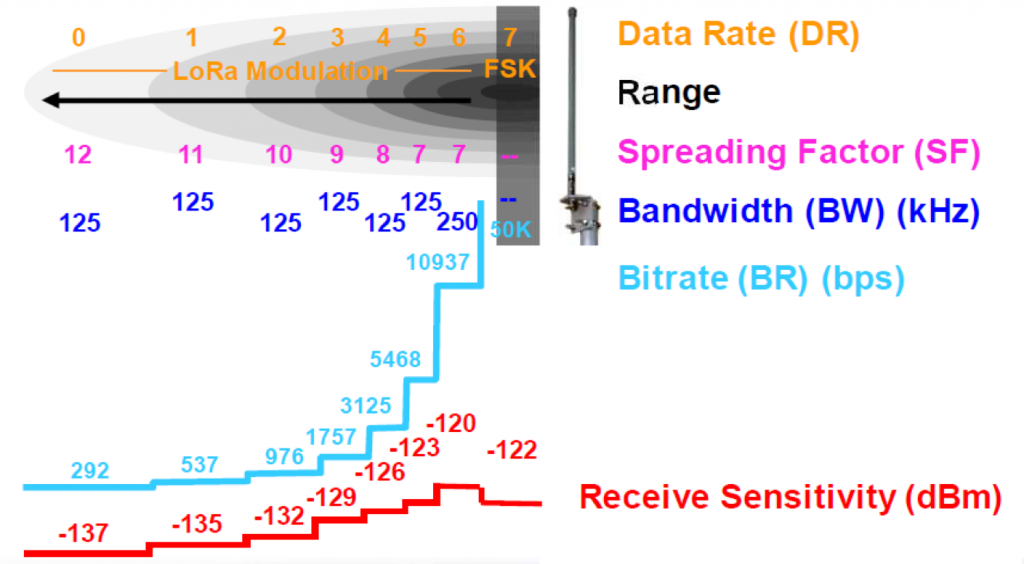
\includegraphics[width=\linewidth]{lorawan_parameters}
    \end{center}
}

\headerbox{3. Genetic Algorithm}{name=model,column=0,below=mcs,span=1}{
    A genetic algorithm is a heuristic search that is used to deal with selection and ranking problems  \cite{vlahogianni_optimized_2005}.
    This algorithm reflects the process of natural selection where the fittest configurations are selected for reproduction in order to produce offspring of the next generation.
    \begin{itemize}
        \item[\ding{224}]  \textbf{Gene:} QoS metric.
        \item[\ding{224}]  \textbf{Chromosome:} QoS of one configuration.
        \item[\ding{224}]  \textbf{Population:} QoS of all configurations.
    \end{itemize}

    \begin{center}
        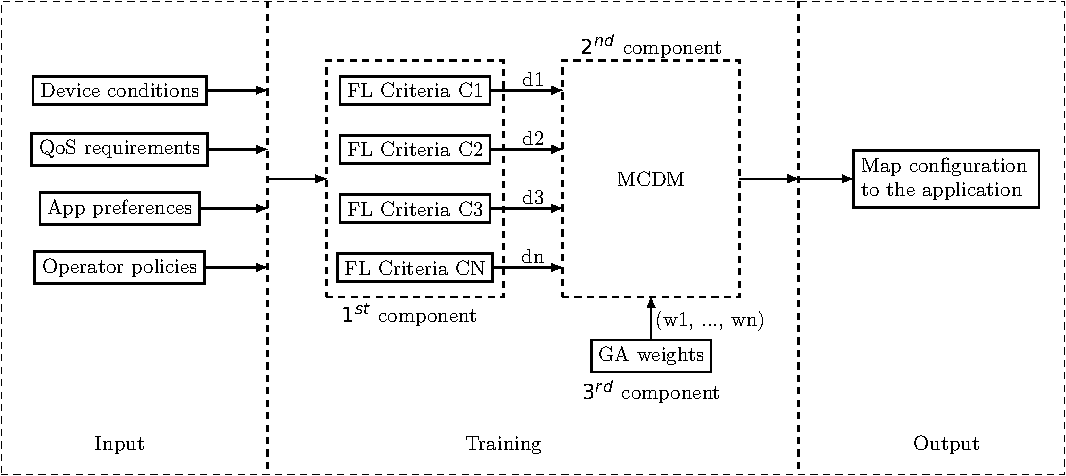
\includegraphics[width=\linewidth]{genetic}
    \end{center}
}

\headerbox{4. LoraWan network}{name=image,span=2,column=1,below=introduction}{
    \begin{center}
        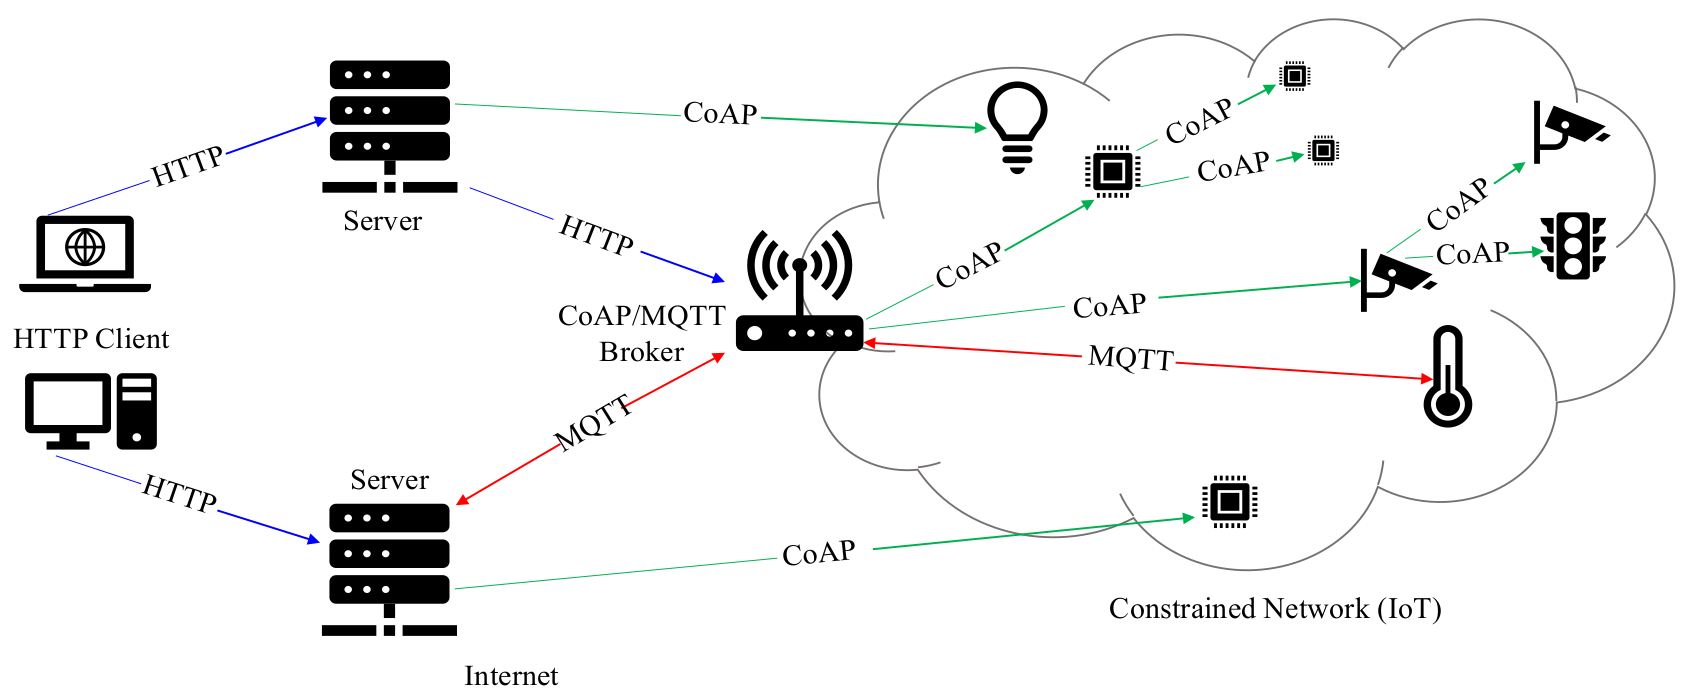
\includegraphics[width=.9\linewidth]{loraI}
    \end{center}
}

\headerbox{5. Algorithm}{name=screen,span=2,column=1,below=image}{
\setlength{\columnsep}{-2.5cm}
    \begin{multicols}{2}
    \textbf{Definition:} stopping criteria, population size P, and mutation probability pm\\
    \textbf{Generate} randomly the initial configurations \\
    \textbf{repeat:}\\
    . . . \textbf{for} each configuration do\\
    . . . . . . Train a model \& compute configuration's fitness\\
    . . . \textbf{end}\\
    . . . \textbf{for} each reproduction 1 ... P/2 do\\
    . . . . . . \textbf{Select:} 2 configurations based on fitness\\
    . . . . . . \textbf{Crossover:} Produce 2 child configurations\\
    . . . . . . \textbf{Mutate:} child configurations with pm\\
    . . . \textbf{end}\\
    \textbf{until} stopping criterion are met\\
    \columnbreak
    \flushright
    \begin{tikzpicture}[node distance=1cm, every node/.style={fill=white, font=\sffamily}, align=center]
      \node (start)       [activityStarts]                     {Parameter initialization};
      \node (fitness)     [selection, below of=start]          {Fitness function};
      \node (crossover)   [selection, below of=fitness]        {Crossover};
      \node (mutation)    [selection, below of=crossover]      {Mutation};
      \node (selection)   [selection, below of=mutation]       {Survivor selection};
      \node (end)         [activityStarts, below of=selection] {Ranked selection list};
  
      \draw[->]     (start)     -- (fitness);
      \draw[->]     (fitness)   -- (crossover);
      \draw[->]     (crossover) -- (mutation);
      \draw[->]     (mutation)  -- (selection);
      \draw[->]     (selection) -- (end);
      \draw[->] (selection.east) to[bend right] (fitness.east);
    \end{tikzpicture}
\end{multicols}

}

\headerbox{6. Experimentation}{name=sea,span=2,column=1,below=screen}{
    In order to generate all the required metrics of each Lora configuration we use both simulation and real environment.
    We use ns3 simulator with 2 nodes and one gateway,
        the distance between each node and the gateway is set to 1km.

    \begin{multicols}{2}
        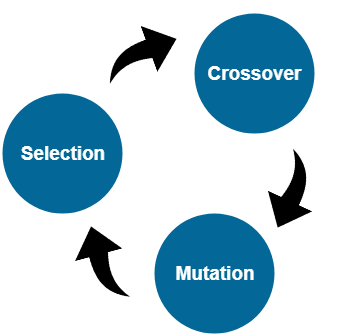
\includegraphics[width=.8\linewidth]{generation}

    \columnbreak
        \bigskip
        \
        \
        \
        \
        \
        \begin{center}
        \begin{tabular}{c|c|c|c}
            \textbf{Setup}   & \textbf{Selection error} & \textbf{Rank} & \textbf{Fitness} \\\hline
            \textbf{1}               & 0.9                      & 1             & 1.5               \\
            \textbf{2}               & 0.5                      & 3             & 4.5               \\
            \textbf{3}               & 0.7                      & 2             & 3                  \\
            \textbf{n}               & 0.5                      & 4             & 6                 \\
        \end{tabular}
        \end{center}

    \end{multicols}

    Results show that genetic algorithm select the configuration that match better the required QoS by the application.
    % In fact,
    %     when we run an application that requires high quality of service,
    %     the algorithm select the configuration that gives large BW and hight data rate with minimum enrgy consumption.
    % When we run an application that requiers less QoS,
    %     the algorithm rank configuration whith sufficient BW and DR.


}

\headerbox{7. Discussion}{name=conclusion,column=1,below=sea,span=2,above=bottom}{

    \ding{224} \textbf{Advantages:}
        Genetic algorithms can manage data sets with many features.
        They don't need specific knowledge about the problem under study.
        These algorithms can be easily parallelized in computer clusters.

    \ding{224} \textbf{Drawbacks:}
        Genetic Algorithms might be very expensive in computational terms,
        since evaluation of each configuration requires building a predictive model.
        These algorithms can take a long time to converge, since they have a stochastic nature.

    \ding{224} \textbf{Conclusion:}
        Genetic algorithms can select the best subset of variables for our predictive model,
        but they usually require a lot of computation but edge computing could solve this problem.

}


\headerbox{7. References}{name=references,column=0,span=1,below=model,above=bottom}{
    \small
    \renewcommand{\section}[2]{\vskip 0.05em} 
    % \bibliographystyle{unsrt}
    \printbibliography
}
\end{poster}